\newpage

\section{Texturas na música}
\index{Música!Texturas}
\label{sec:texturasmusica}
\begin{wrapfigure}{r}{0.33\textwidth}
    \centering 
    \vspace{-10pt}
    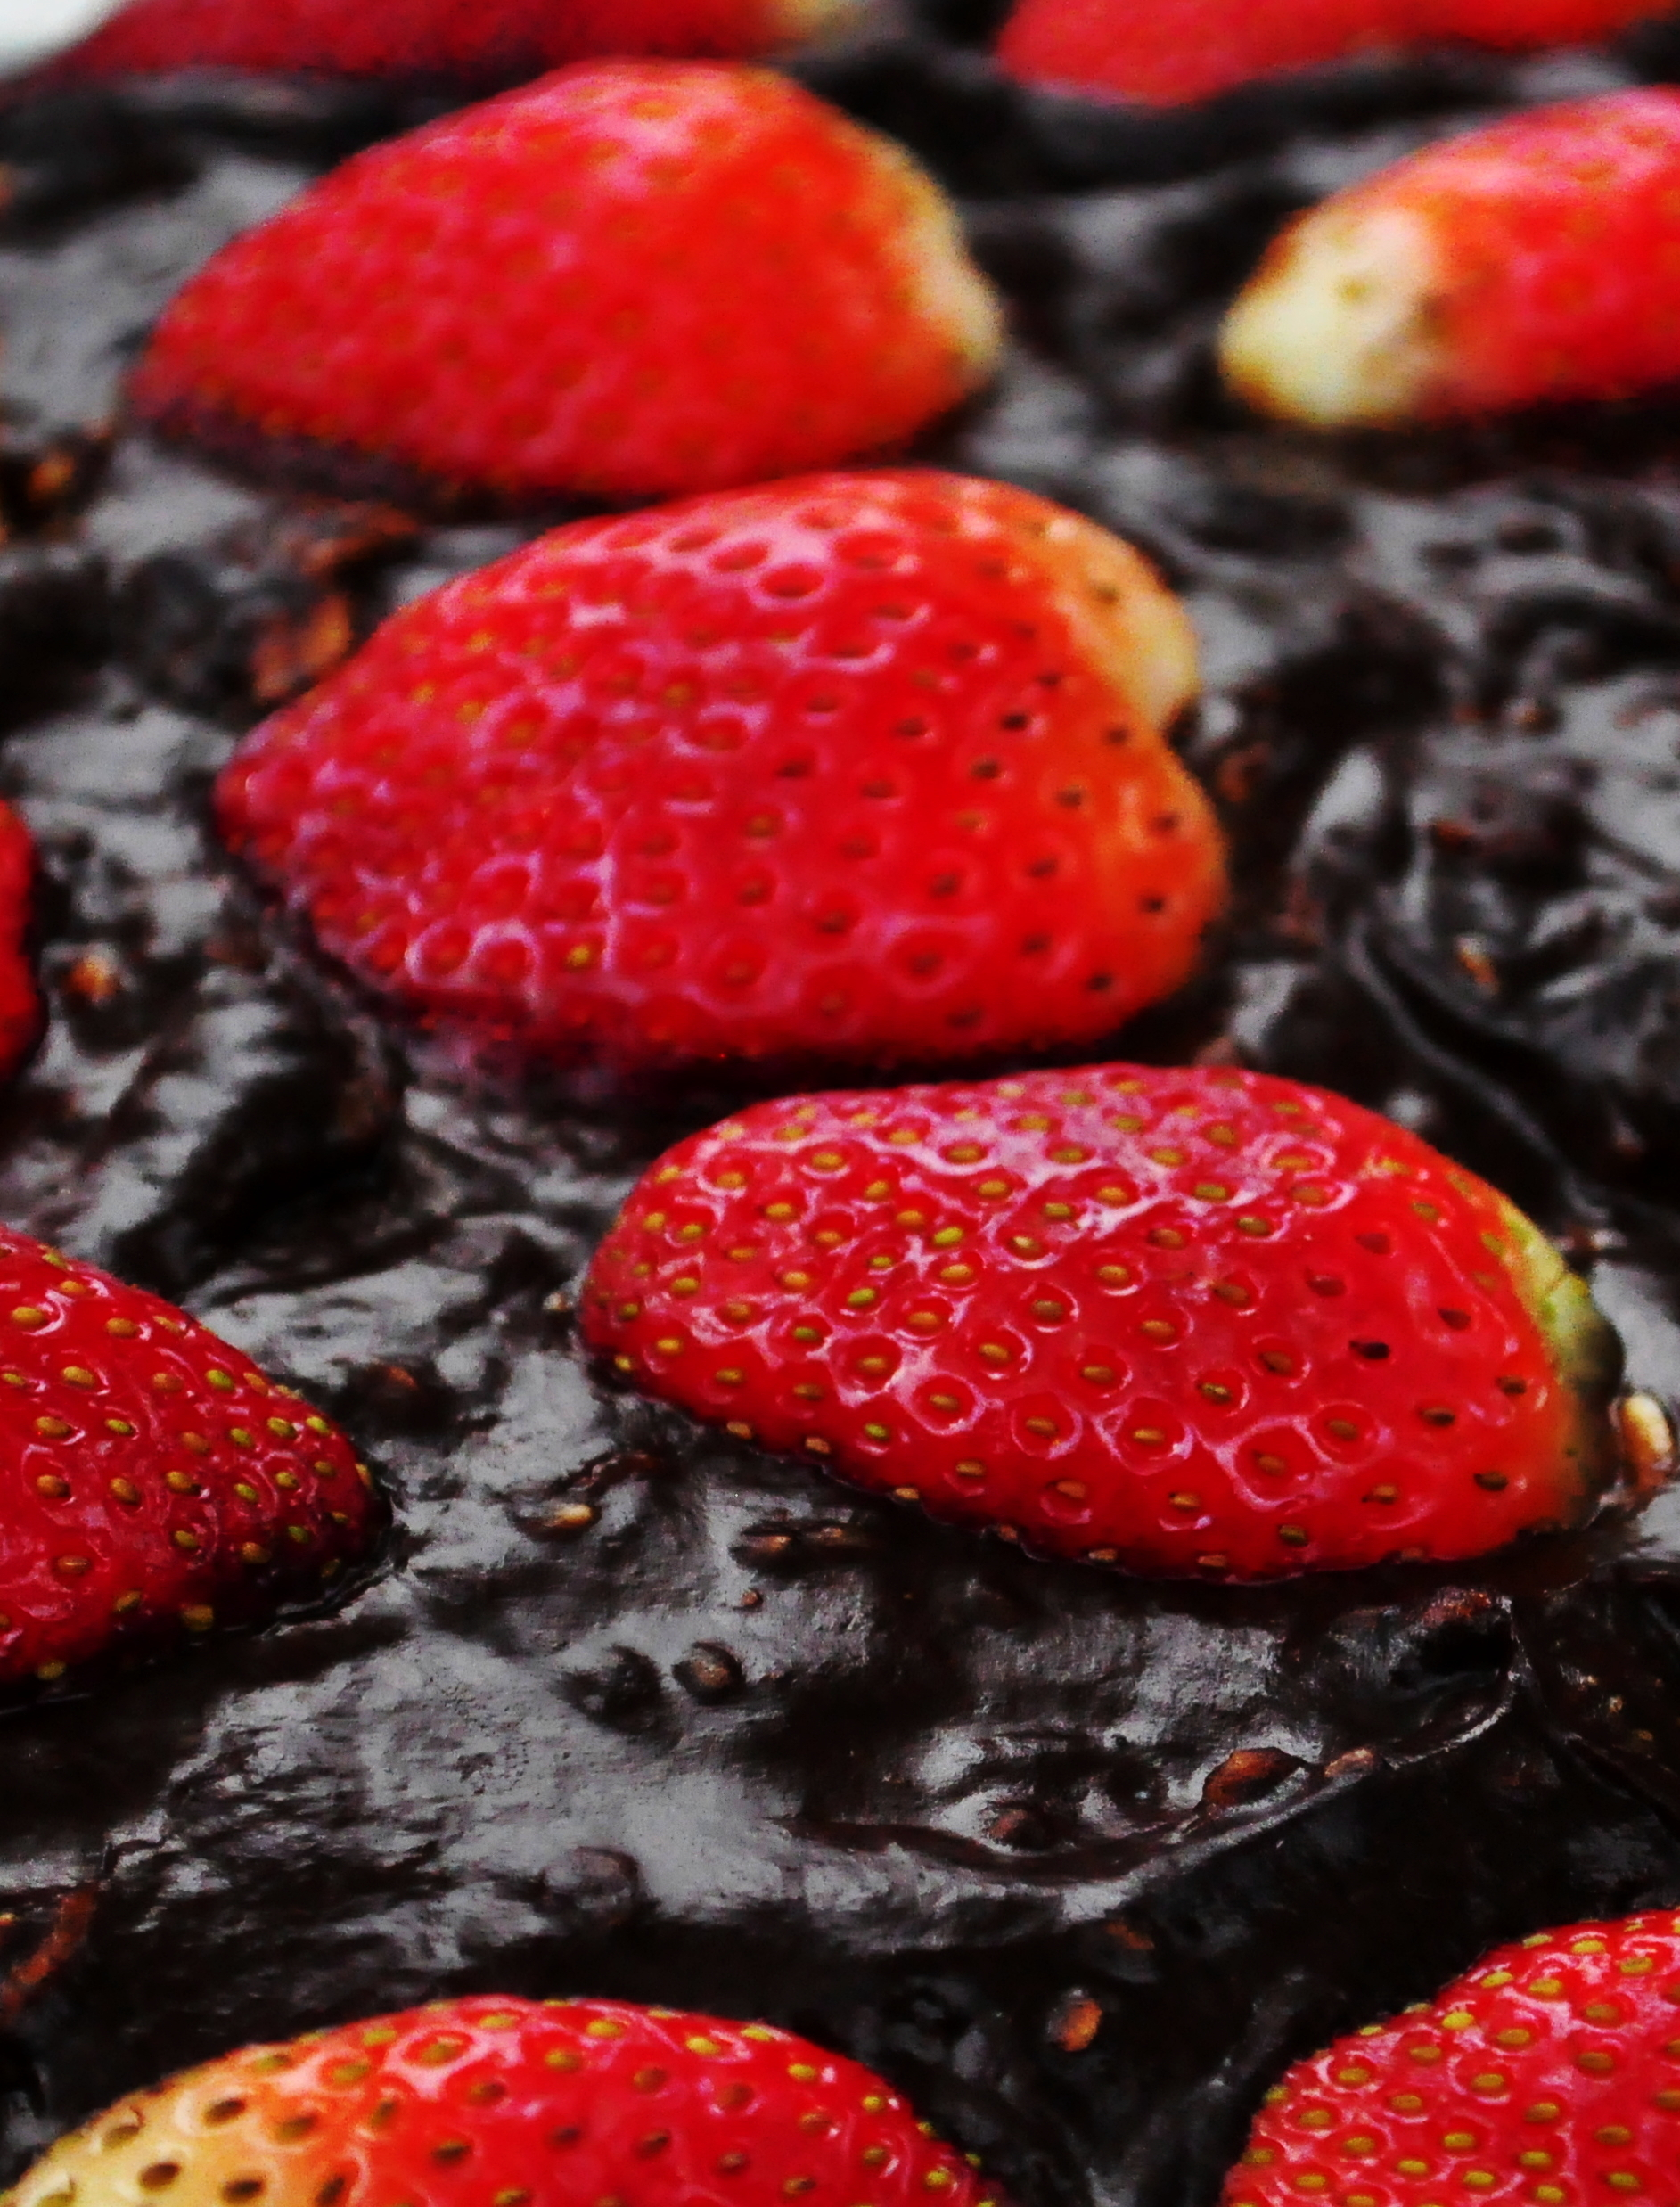
\includegraphics[width=0.30\textwidth]{chapters/cap-musicalidade-percepcion/textura.jpg}
  \caption{Texturas.}
    \vspace{-10pt}
\end{wrapfigure}
De forma similar a como descrevemos a textura numa superfície,
podemos explicar a textura na música.
A textura musical é um termo usado para indicar o modo em que interagem e 
se misturam várias linhas melódicas \cite[pp. 29]{kerman2015listen}.


O termo textura usado na música, 
implica que esta é composta por instrumentos com a capacidade de gerar tons,
e consequentemente melodias;
dado que a percussão não é geralmente considerada como melódica, 
esta não é tomada em conta quando usamos o termo textura \cite[pp. 59]{holland2013music}.

Na música atual existem  vários tipos de texturas, 
porém 3 destes tipos  são os mais comuns 
\cite[pp. 77]{copland1974ouvir} \cite[pp. 29]{kerman2015listen} \cite[pp. 322]{harnum2009basic}:
\begin{inparaitem}
\item textura monofônica, 
\item textura homofônica e
\item textura polifônica.
\end{inparaitem}

 
%%%%%%%%%%%%%%%%%%%%%%%%%%%%%%%%%%%%%%%%%%%%%%%%%%%%%%%%%%%%%%%%%%%%%%%%%%%%%%%%
\subsection{A textura monofônica}
\label{subsec:monofonica}
\index{Música!Monofônica}
\begin{wrapfigure}{r}{0.33\textwidth}
\centering
    \vspace{-10pt}
    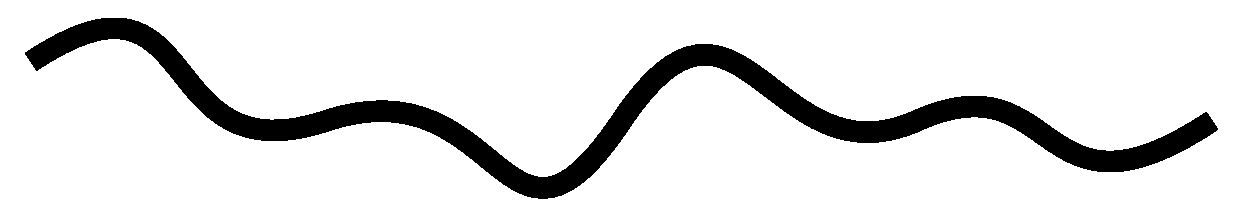
\includegraphics[width=0.31\textwidth]{chapters/cap-musicalidade-percepcion/monofonica1.eps}
  \caption{Textura monofônica.}
\end{wrapfigure}
Este tipo de música tem uma única linha melódica sem acompanhamento.
Consequentemente este tipo de música é a mais simples de ouvir, 
pois nossa atenção cai sobre uma única camada na música \cite[pp. 77]{copland1974ouvir} \cite[pp. 29]{kerman2015listen}.
A música monofônica corresponde ao tipo mais antigo de música \cite[pp. 539]{apel1969harvard}.
Se considera que é uma textura monofônica, mesmo que sejam muitas vozes as que executem uma mesma melodia, 
ou que estas executem a mesma melodia em oitavas diferentes \cite[pp. 42]{bennett1993elementos} \cite[pp. 58]{holland2013music}.

A qualificação de textura  monofônica não é afetada pelo uso de instrumentos de percussão tocando junto com a melodia;
a textura monofônica refere-se à parte tonal da música, é dizer à melodia, 
não à textura rítmica da música \cite[pp. 58]{holland2013music}.

\begin{example}
A Figura \ref{fig:ex:monofonica} mostra um exemplo de uma seção de música com textura monofônica.
\end{example}

\begin{figure}[!h]
\centering
    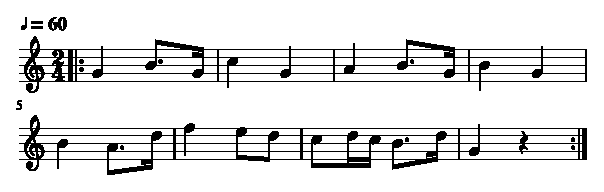
\includegraphics[width=0.99\textwidth]{chapters/cap-musicalidade-percepcion/textura-monofonica-1.eps}
  \caption{Textura monofônica.}
\label{fig:ex:monofonica}
\end{figure}
 
\begin{example}
Um exemplo, no ocidente,  muito depurado de música monofônica é o canto gregoriano
\cite[pp. 77]{copland1974ouvir} \cite[pp. 29]{kerman2015listen} \cite[pp. 58]{holland2013music}. 
Aqui, não importa o número de vozes usadas na interpretação,
pois todas seguem a mesma linha melódica, pelo que é considerada uma textura monofônica.
\end{example}

%monodia \cite[pp. 38]{schurmann1989m} 

%%%%%%%%%%%%%%%%%%%%%%%%%%%%%%%%%%%%%%%%%%%%%%%%%%%%%%%%%%%%%%%%%%%%%%%%%%%%%%%%
\subsection{A textura homofônica}
\label{subsec:homofonica}
\index{Música!Honofônica}
\begin{wrapfigure}{r}{0.33\textwidth}
  \centering
    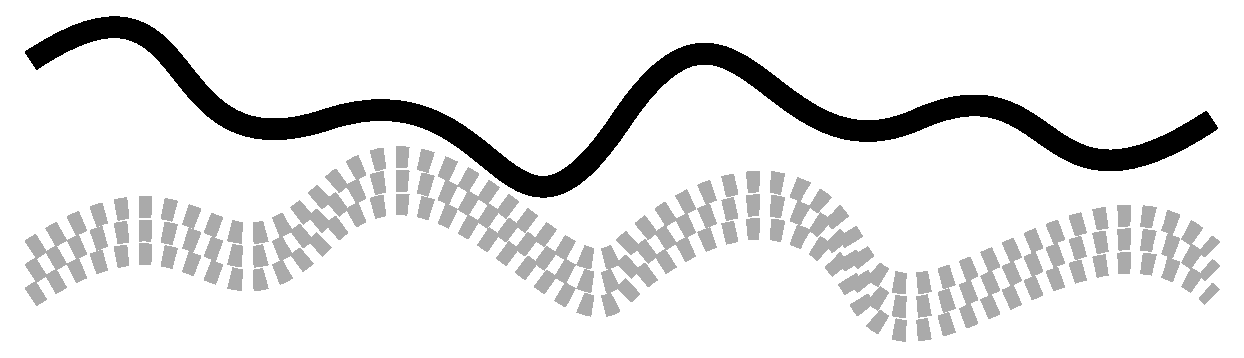
\includegraphics[width=0.31\textwidth]{chapters/cap-musicalidade-percepcion/honofonica1.eps}
  \caption{Textura homofônica.}
\end{wrapfigure}
O termo ``homofônico'' ou ``homofonia'' significa literalmente ``vozes semelhantes''.%% Falta referença
A textura homofônica consiste de uma linha melódica principal e um acompanhamento por acordes,
de modo que existe uma distinção clara entre a melodia e a harmonia de acompanhamento;
esta textura é o tipo  mais usado na música atual,
e só é ligeiramente mais complexa que a textura monofônica 
\cite[pp. 78]{copland1974ouvir} \cite[pp. 29]{kerman2015listen} 
\cite[pp. 43]{bennett1993elementos} \cite[pp. 58]{holland2013music}.


A homofonia é o oposto da polifonia, 
pois na textura homofônica só uma linha melódica é importante,
enquanto que na textura polifônica todas as partes contribuem equitativamente para gerar o tecido musical
\cite[pp. 687]{apel1969harvard}.

\begin{example}
A Figura \ref{fig:ex:homofonica} mostra um exemplo de uma seção de música com textura homofônica.
\end{example}

\begin{figure}[!h]
\centering
    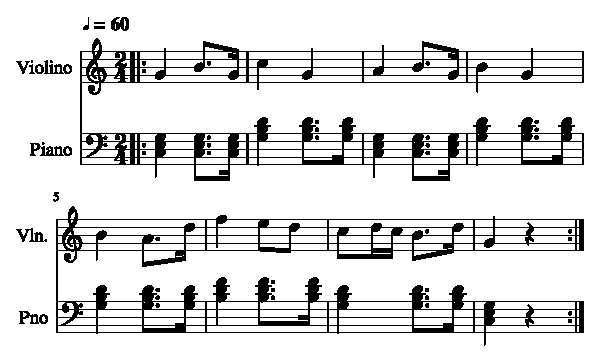
\includegraphics[width=0.99\textwidth]{chapters/cap-musicalidade-percepcion/textura-homofonica-1.eps}
  \caption{Textura homofônica.}
\label{fig:ex:homofonica}
\end{figure}

\begin{example}
Um exemplo de textura homofônica pode ser visto no choro ``Deixe o breque pra mim'',
de Altamiro Carrilho, 
onde a melodia principal é feita por um único instrumento (flauta), 
com uma base harmônica e percussiva, de acompanhamento.
\end{example}

%\cite[pp. 121]{schurmann1989m} 


%%%%%%%%%%%%%%%%%%%%%%%%%%%%%%%%%%%%%%%%%%%%%%%%%%%%%%%%%%%%%%%%%%%%%%%%%%%%%%%%
\subsection{A textura polifônica}
\index{Música!Polifônica}
\label{subsec:polifonica}
\begin{wrapfigure}{r}{0.33\textwidth}
\centering
    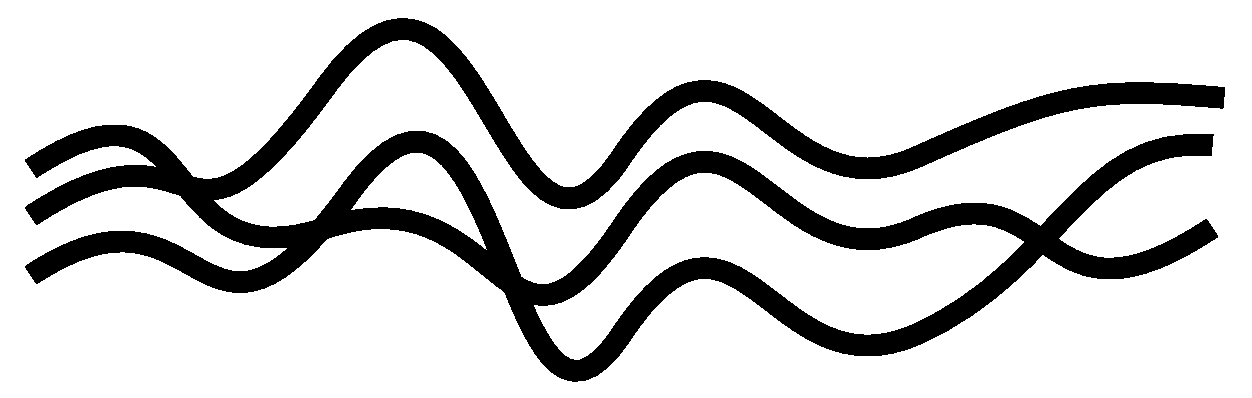
\includegraphics[width=0.31\textwidth]{chapters/cap-musicalidade-percepcion/polifonica1.eps}
  \caption{Textura polifônica.}
\end{wrapfigure}
Termo proveniente do grego, que significa ``vozes múltiplas''.%% Falta referença
A música com textura polifônica se carateriza por ter duas ou mais linhas melódicas, 
que se entrelaçam continuamente;
as melodias são consideradas independentes e de interesse aproximadamente igual.
A percepção da música polifônica precisa de um maior nível de atenção, 
em comparação das texturas monofônica e homofônica,
pois exige ao ouvinte a capacidade de separar mentalmente cada linha melódica  
\cite[pp. 79-80]{copland1974ouvir} \cite[pp. 29]{kerman2015listen} 
\cite[pp. 42]{bennett1993elementos} \cite[pp. 59]{holland2013music}
\cite[pp. 687]{apel1969harvard}.

Uma termo frequentemente usado na música polifônica é o contraponto;
que é a técnica de escrever duas ou mais melodias que se encaixam 
\cite[pp. 29]{kerman2015listen} \cite[pp. 42]{bennett1993elementos}.

\begin{tcbinformation}{Quantas vozes independentes pode captar simultaneamente um ser humano?}
\label{ref:quantasvozes}
Não existe um senso comum, porém pode-se afirmar que treinando um pouco,
é possível perceber independentemente 2 ou 3 vozes sendo executadas em simultâneo \cite[pp. 81]{copland1974ouvir}. 
\end{tcbinformation} 

\begin{example}
Um exemplo de textura homofônica pode ser visto na música ``Canto e Contraponto'',
de Toquinho e Vinícius, 
onde temos uma melodia executada pela voz, e outra melodia executada por um instrumento fazendo o contraponto, 
com uma base harmônica de acompanhamento.
\end{example}

\begin{example}
A Figura \ref{fig:ex:polifonica} mostra um exemplo de uma seção de música com textura polifônica.
\end{example}

\begin{figure}[!h]
\centering
    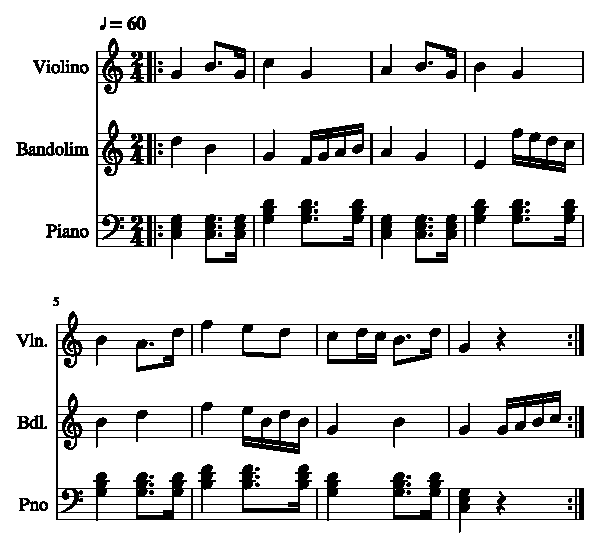
\includegraphics[width=0.99\textwidth]{chapters/cap-musicalidade-percepcion/textura-polifonica-1.eps}
  \caption{Textura polifônica.}
\label{fig:ex:polifonica}
\end{figure}



%\cite[pp. 64]{schurmann1989m} 

%%%%%%%%%%%%%%%%%%%%%%%%%%%%%%%%%%%%%%%%%%%%%%%%%%%%%%%%%%%%%%%%%%%%%%%%%%%%%%%%
\subsubsection{Polirritmia}
\index{Música!Polirritmia}
\label{subsec:polirritmia}
A polirritmia é a superposição de dois ou mais ritmos.
A polirritmia acontece quando se executam musicas com texturas polifônicas ou homofônicas
\cite[pp. 93]{alves2004teoria};
ou quando vários instrumentos de percussão tocam ritmos diferentes simultaneamente \cite[pp. 35]{holland2013music}.
Assim, a textura dos ritmos simultâneos é chamada polirritmia \cite[pp. 35]{holland2013music}.

Cada instrumento de percussão ``fala'' um ritmo único que geralmente guia os passos e movimentos dos dançarinos;
por exemplo, a música africana é conhecida por ter múltiplas camadas de ritmo e sincopas,
 que são usadas continuamente pelos dançarinos \cite[pp. 35]{holland2013music}.


É possível distinguir dois tipos de polirritmia \cite[pp. 687]{apel1969harvard}:
\begin{itemize}
\item Ritmos contrastantes dentro da mesma \hyperref[def:Metrica]{\textbf{métrica}};
por exemplo, os ritmos mostrados na Figura \ref{fig:polirritmia1-1}.
\begin{figure}[!h]
\centering
    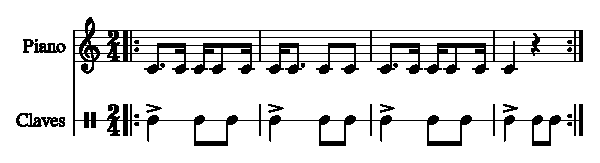
\includegraphics[width=\textwidth]{chapters/cap-musicalidade-percepcion/polirritmia1-1.eps}
  \caption{Textura polirrítmica com a mesma métrica.}
\label{fig:polirritmia1-1}
\end{figure}
\item Ritmos contrastantes com diferente \hyperref[def:Metrica]{\textbf{métrica}} ou acentuações, 
às vezes é denominado ``polimétrico'';
por exemplo, os ritmos mostrados na Figura \ref{fig:polirritmia2-1}.
\begin{figure}[!h]
\centering
    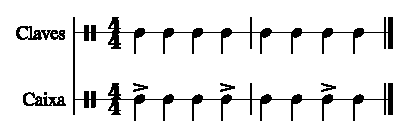
\includegraphics[width=0.7\textwidth]{chapters/cap-musicalidade-percepcion/polirritmia2-1.eps}
  \caption{Textura polirrítmica com diferente métrica.}
\label{fig:polirritmia2-1}
\end{figure}
\end{itemize}


